\documentclass{article}

\usepackage{graphicx}
\usepackage{latexsym}

\setlength{\pdfpagewidth}{8.5truein}
\setlength{\pdfpageheight}{11truein}

\def\s{\hbox{s}}
\def\m{\hbox{m}}

\usepackage{fullpage}

\addtolength{\topmargin}{-.5in}
\textheight 9in

\begin{document}

\title{Physics and Math of Music --- Day 2 --- The ear}
\date{Tuesday, February 5, 2002}
\author{Peter Folk ({\tt pfolk@uni}) and Paul Grayson ({\tt pgrayson@uni})}
\maketitle

\section*{Many oscillators resonating}
When you shake one pendulum back and forth at its natural frequency,
it resonates.  Now, what happens when you shake more than one pendulum
at the same time?  The ones that have a natural frequency that matches
the shaking will start swinging; the other ones won't.  So, if we have
pendulums of {\sl many\/} different frequencies, we can identify the
frequency of shaking just by checking which pendulums are moving.
That's how your ear works!

\section*{A model of the ear}
The ear detects the frequency of sound by using thousands of
little oscillators.  Figure~\ref{ear} shows how this works:

\begin{figure}[h]
\begin{center}
	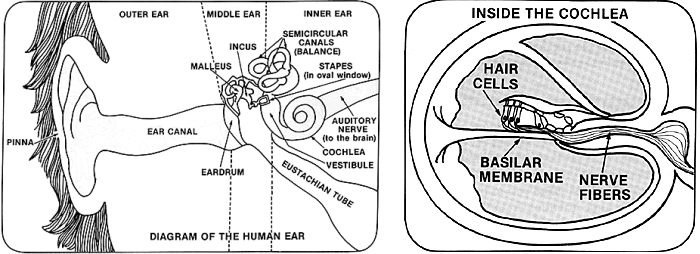
\includegraphics[width=4in]{figures/ear2.png}
	\caption{On the left is a view of the inside of your ear.  On the right is a
	cross-section of the cochlea, where sound is detected by tiny hair
	cells --- resonating oscillators! Thanks to
	{\tt http://clerccenter.gallaudet.edu/InfoToGo/535/535-1.html} for
	the nice ear pictures.}\label{ear}
\end{center}
\end{figure}

Each one of those little hair cells is an oscillator, just like one of
our pendulums.  The force that shakes them comes in from the air: if a
hair has a natural frequency matching a sound in the air, it starts
vibrating.

\section*{Multiple frequencies at the same time}
A sound is made up of many different frequencies, and our ears allow
us to hear them all.  Once you know all of the frequencies in a
sound\footnote{To perfectly recreate the sound, you would also need
the {\it phases} of all of the frequencies --- something a microphone
can measure but our ears can't.}, you know everything about the sound.
This measurement of the frequencies that make up a wave is called a
{\it Fourier transform}.  It is so useful to look at the frequencies
of a wave that the Fourier transform is used for everything; from
encoding your \verb^mp3^s and cleaning up musical recordings to
matching up fingerprints for the FBI.

\begin{figure}[h]
\begin{center}
	\input figures/sine_wave.tex
	\caption{Plot of a simple sine wave: $x = A \sin(2\pi f t)$. }
	\label{sine_wave}
\end{center}
\end{figure}
\begin{figure}[h]
\begin{center}
	\input figures/sine_wave.f.tex
	\caption{The response of your ear to a simple sine wave ---
	just a few hairs oscillate.}
	\label{sine_wave.f}
\end{center}
\end{figure}

\begin{figure}[h]
\begin{center}
	\input figures/piano_note.tex
	\caption{Plot of more complicated wave: the sound of a note on
	a piano. }
	\label{sine_wave}
\end{center}
\end{figure}
\begin{figure}[h]
\begin{center}
	\input figures/piano_note.f.tex
	\caption{The response of your ear to a piano note ---
	many different hairs oscillate.  Their oscillations will also
	change over time as the note decays.}
	\label{sine_wave.f}
\end{center}
\end{figure}

\end{document}
